
%%%%%%%%%%%%%%%%%%%%%%%%%%%%%%%%%%%%%%%%%%%%%%%%%%%%%%%%%%%%%%%%%%%%%%%%%
%           Capítulo 3: NOMBRE                   %
%%%%%%%%%%%%%%%%%%%%%%%%%%%%%%%%%%%%%%%%%%%%%%%%%%%%%%%%%%%%%%%%%%%%%%%%%

\chapter{Estudio de las poblaciones estelares}

\lettrine[lines=1]{E}n este capitulo analizaremos las poblaciones estelares de UGC11680 y así mismo estudiaremos el enrojecimiento por polvo y la tasa de formación estelar.

\section{Espectroscopía De Campo integral}

La espectroscopía de Campo Integral (de aquí en delante IFS por sus siglas en
inglés, \textit{Integral Field Spectroscopy}) es una técnica de observación astronómica capaz de obtener simultáneamente y en una sola
exposición espectros de típicamente muchos elementos espaciales (\textit{spaxels}) de una fuente sobre un campo de visión bidimensional.
Un espectrógrafo de campo integral consiste de dos componentes: el espectrógrafo y la unidad de campo integral (IFU por sus siglas en inglés, \textit{Integral Field Unit}) cuya función es dividir el plano espacial 2D en un arreglo de \textit{spaxels}
individuales y dirigir el haz de luz de cada uno de ellos al espectrógrafo, de manera que obtenemos una gran cantidad de imágenes
cada una a diferente longitud de onda. En general, todas ellas pueden formar un cubo de datos con la información
en tres dimensiones, dos espaciales $X$, $Y$ (declinación y ascensión recta) y longitud de onda. Ver Figura \ref{cubo}


\begin{figure}
  \centering
    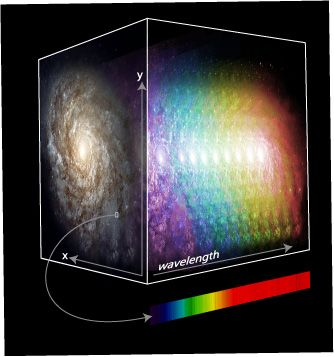
\includegraphics[scale=0.5]{data-cube-illustration.jpg}
  \caption[Cubo de Datos]{Representación esquemática de un cubo de datos.}
  \label{cubo}
\end{figure}

\subsection{CALIFA}

El \textit{Calar Alto Legacy Integral Field Area Survey} (\textbf{CALIFA}) \citep{sanchez2012}
fue un  proyecto  del Centro Astronómico Hispano-Alemán en el Observatorio de Calar Alto para
obtener espectros espacialmente resueltos de 600 galaxias del Universo Local ($0.005 <z <0.03$)
por medio de espectroscopía de campo integral (IFS). Las observaciones en \textbf{CALIFA}
comenzaron en junio de 2010 con el espectrografo Multi-Apertura Postdam (PMAS), montado en un telescopio de 3-5m,
utilizando  campo de visión hexagonal (FOV) \citep{Verheijen2004}.

\bigskip

\noindent En este espectrógrafo, se observó cada galaxia usando dos configuraciones diferentes,
una resolución del intermedio espectral (V 1200, R $\sim$ 1650) que cubre la gama del azul en el óptico (3700-4700 \text{\AA})
y una de baja resolución  (V 500, R$\sim$ 850) que cubre el primer orden de la longitud de onda óptica (3750-7500 \text{\AA}.
(Para este trabajo se utilizó los cubos de datos del V500).

\bigskip


\noindent Una muestra seleccionada  de 939 galaxias se extrajo de la séptima publicación de los datos del SDSS,
que es se describe en \citep{walcher2014}. A partir de esta muestra, 600 galaxias son seleccionadas al azar.
La combinación de técnicas de imagen y espectroscopía óptica a través de IFS proporciona una visión más completa de propiedades
de las galaxias individuales que cualquier survey tradicional y en comparación con otros surveys IFS, \textbf{CALIFA} ofrece para nuestro caso las siguientes características:


\begin{itemize}

\item Una muestra que abarca una amplia gama de tipos morfológicos, cubriendo toda la secuencia de Hubble , desde elípticas (E0-E7), lenticulares (S0-S0a) a espirales, además de un amplio rango de masas ($10^9$ $\sim$ $10^{12}$ $M_{\odot}$)

\item Una muestra que cubre todo el  diagrama color-magnitud para $M_r > - 18$ mag que nos permite obtener relativamente bien las poblaciones galácticas (secuencia roja, nube azul y valle verde);

\item Observaciones que cubren el rango la longitud de onda  del espectro óptico, que nos permite obtener la historia de formación estelar para las poblaciones estelares subyacentes.

\end{itemize}

\noindent En artículos previos con esta muestra, y usando las historias de formación estelar de $\sim$ 100 galaxias \citep{perez2013} derivaron la información espacialmente resuelta del crecimiento de masa galáctica. Además, \citep{gonzalez2014} describieron  las propiedades de las poblaciones estelares. Ambos artículos confirmaron que las galaxias masivas acumulan su masa estelar de dentro hacia afuera. Encontraron además que las galaxias más masivas eran más compactas, viejas, mas ricas en metales y menos enrojecidas por polvo.
De esta forma usaremos varios de estos métodos descritos en estos y otros trabajos con la muestra de \textbf{CALIFA}.

\subsection{Enrojecimiento por Polvo}

Antes de avanzar en el estudio de las poblaciones estelares de la galaxia UGC11680,
revisamos la atenuación por polvo en ella, ya que es posible
que solo sea este lo que la vuelve mas roja. Para cuantificar el nivel de
extinción en UGC11680 comparamos en su espectro integrado la diferencia en flujo en las primeras dos
linea de la secuencia de Balmer ($H\alpha$ y $H\beta$). La razón esperada entre los flujos de estas dos líneas
es de $R_{int}=F\alpha/F\beta=2.86$ \citep{osterbrock1989}. Por lo tanto, desviaciones de esa relación se pueden usar para medir
la extinción relativa entre $H\alpha$ (a 6562.8 \text{\AA} en la banda r) y $H\beta$ (a 4861 \text{\AA} en la banda g).

\begin{figure}
  \centering
    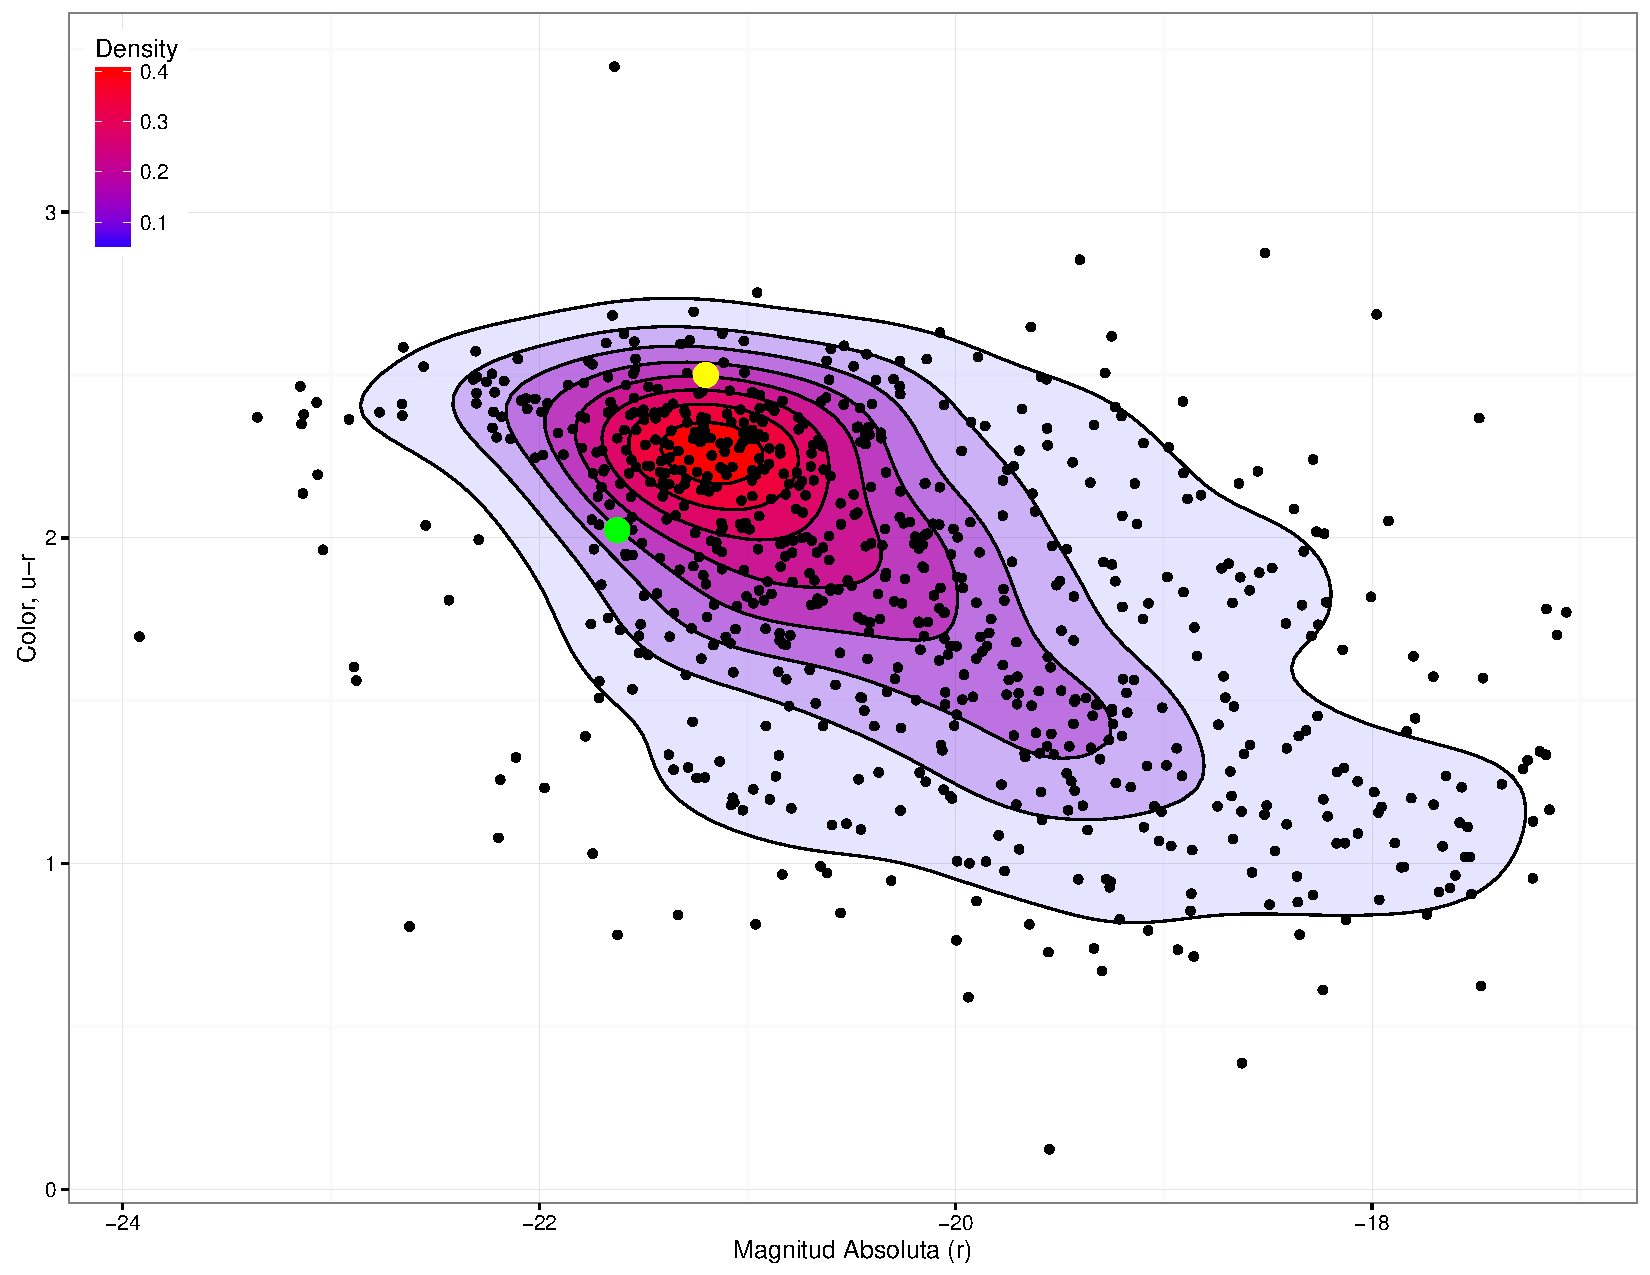
\includegraphics[scale=0.5]{color_magnitud_ur.pdf}
  \caption[Diagrama Color-Magnitud con UGC11680]{Diagrama en Color Magnitud para las galaxias de la muestra de  \textbf{CALIFA}. Marcamos las posiciones de la galaxia UGC11680 por dos puntos. El punto amarillo representa a UGC11680 sin corregir por polvo y el punto verde lo muestra ya corregido. Nótese que a pesar de que el polvo la enrojece, ese enrojecimiento no es suficiente para sacarla de la secuencia roja.}
  \label{cmd1}
\end{figure}


\noindent A raíz de la relación de extinción empírica, las luminosidades intrínsecas, $L _{int}$, están dadas por

\begin{equation}
L _{int} (\alpha) = L_{obs} (\lambda) 10^{0.4A_{\lambda}} =L_{obs} (\lambda) 10^{0.4k(\lambda)E(B-V)}
\end{equation}

\noindent donde $L_{obs}$ son las luminosidades (extinguidas) observadas, $A(\lambda)$ es la extinción a la longitud de onda $\lambda$,
 y $k(\lambda)$ de la curva de enrojecimiento.El exceso de color se define por

\begin{equation}
E(B -V) =(B - V)_{obs}-(B - V)_{int}
\end{equation}

\noindent que es el cambio en el  color $(B - V)$  debido al polvo (es decir, la diferencia entre el color observado y esperado
en ausencia de polvo). El decremento de Balmer intrínseco se mantiene constante para condiciones típicas de gas \citep{osterbrock1989}, por lo que


\begin{equation}
E(H\beta - H\alpha) = 2.5 \log \frac{F_{obs}}{F_{int}},
\end{equation}





\noindent y por lo tanto un calculó con los datos obtenidos del cubo de datos perteneciente a la galaxia UGC11680 que se muestran en
la tabla \ref{tab_valores} nos da finalmente una  $A_V \sim 1$ mag. El resultado se muestra con el diagrama de color magnitud de la Figura \ref{cmd1}. La posición de UGC11680 se muestra con puntos en el diagrama y su corrección también se muestra en este. El diagrama también muestra la secuencia roja  en nuestra muestra. Hay que notar que la galaxia UGC11680 perdió posición dentro de esta densidad corregida, sin embargo no es suficiente para que salga de la secuencia roja.


\bigskip


\noindent Esto nos da una idea de lo que esta pasando. En general, \citep{sanchez2012} para las galaxias de cara con morfología Sb-Scd, la extinción esta en el rango de $A_V \sim 1.3$ mag. Así, La galaxia UGC11680 tiene un valor relativamente normal de extinción para las galaxias de su tipo y se encuentra dentro de los rangos comunes para las galaxias de cara y no es suficiente para sacarla de la secuencia roja de la muestra y así lo indica la Figura \ref{cmd1}. Esto ya elimina la extinción como causante de que UGC11680 se encuentre en la secuencia roja.





\subsection{Tasa de formación estelar}

La tasa de formación estelar (SFR) es la masa de gas convertido en estrellas por unidad de tiempo.
La unidad estándar para medir el SFR es la masa solar por año ($M_{\odot}/ yr$). La SFR puede
medirse en pequeñas regiones de una  galaxia, como una nube molecular única, en
galaxias, y en todo el universo. La SFR a un \textsl{redshift} dado es un elemento esencial de
información sobre la evolución de una determinada galaxia o toda la población de ellas
en ese tiempo. Seguir la SFR en el tiempo es equivalente a seguir el ensamblaje de la masa estelar
en el universo. Hay varios métodos empíricos para estimar el SFR desde el ultravioleta, óptico,
y a partir de observaciones en el infrarrojo. Todos los métodos se basan en la teoría estándar de formación de estrellas
 y emplea diferentes tipos de emisión asociados a este tipo de eventos.

 \begin{figure}
  \centering
    \includegraphics[scale=0.5]{sfr_califa2.pdf}
  \caption[Diagrama de Tasa de Formación estelar]{Tasa de Formación estelar con respecto a
           la masa estelar para la muestra de \textbf{CALIFA} en escala logarítmica. En este diagrama La posición de la galaxia
          UGC11680 dentro del diagrama se marca con el punto azul. En este diagrama se observa lo reportado en \cite{cano2016}, la existencia de dos secuencias: la de las galaxias formadoras de estrellas y las retiradas. Nótese que la galaxia UGC11680 se encuentra debajo de la secuencia de galaxias formadoras de estrellas y sobre la secuencia de las retiradas. }
  \label{sfr_califa}
\end{figure}


\bigskip

\noindent En \citep{sanchez2013} se derivó la tasa de formación estelar sumando los flujos de $H \alpha$ de las regiones $HII$ dentro del campo de visión de las galaxias de la muestra de \textbf{CALIFA}, con atenuación por polvo usando una extinción promediada derivada de esas regiones. Aunque hay una discrepancia entre las tasas derivadas, aquí se asume una tasa de formación de \citep{kennicutt1998}


\begin{equation}
SFR(Myr^{-1})= 7.9 \times 10^{-42} L_{H_{\alpha}} (\text{erg} \text{s}^{-1})
\label{tasa}
\end{equation}



\noindent Para el caso de la galaxia UGC11680 la tasa de formación estelar estimada con esta relación resultó ser $\log$ $SFR$ $\sim$ 0.6 $\log_{10}$ $(M_{\odot}/yr^2)$ ó $SFR \sim $  4.1 ($M_{\odot}/yr^2$).

\subsection{La secuencia de galaxias formadoras de estrellas}

Una de las formas de visualizar la propiedades de evolución de las galaxias es graficar la SFR contra la masa estelar $M_{*}$
para todas las galaxias de la muestra. Tal diagrama se muestra en la Figura \ref{sfr_califa} y sobresalen dos cosas. Una, la secuencia que contiene a las las galaxias que forman estrellas. A las galaxias que están concentradas en esa secuencia a veces se le llama galaxias de secuencia principal ó galaxias SF; segundo, la secuencia debajo de la SF, que es conocida como de las galaxias retiradas o galaxias que en su mayoría dejaron de formar estrellas.

\bigskip

\noindent En \citep{cano2016} se reporta un valor de 0.81 en la pendiente de galaxias formadoras de estrellas en la muestra de \textbf{CALIFA}. Para nuestro caso y con los datos dados en la
introducción, encontramos un valor de $\beta=0.83$ donde $\beta$  es la pendiente de la relación. En ese mismo artículo
se encuentra que las galaxias retiradas tienen una pendiente de $\beta \sim 0.86$  por lo que coloca a UGC11680 en el
lugar entre las galaxias retiradas y las galaxias en la SF. Es interesante notar que  UGC11680 se encuentra entre estas dos secuencias en la Figura \ref{sfr_califa}. Esto implica que  UGC11680, deja de formar estrellas pero no completamente, lo que podría ser un indicador de que el AGN de UGC11680 es un tipo de regulador de formación estelar. Esta implicación podría tener consecuencias relevantes en el estudio que sigue.



\section{Análisis de poblaciones estelares}

La masa también es un factor fundamental en la evolución galáctica. Como se mencionó en la introducción, la mayor parte de las galaxias se han formado a través de fusiones e interacciones de forma jerárquica, es decir, pequeños sistemas se han fusionado para formar sistemas más grandes. A épocas cosmológicas tempranas, la formación estelar era más efectiva en galaxias masivas pero en épocas cosmológicas más recientes la formación estelar se apagó en galaxias masivas, pero continuó en galaxias más pequeñas ,un fenómeno llamado ahora ``downsizing'' \citep{corteau2014} ({\color{red} Ibarra-Medel, et al. Submitted }).

\bigskip

\noindent Así mismo, las galaxias brillan por que sus estrellas radian la energía que producen por reacciones nucleares en sus centros. La teoría de evolución estelar describe la cantidad de energía liberada  por una estrella dada su masa inicial. Entonces, modelando la luz emitida por todas sus estrellas en una galaxia sobre todas sus longitudes de onda se obtiene la llamada ``distribución de energía espectral'' (SED), y así se puede derivar (en principio) la masa estelar que es responsable de esa radiación. Históricamente, como había sido señalado por Baade \citep{baade1957}, nuestra propia Vía Láctea esta compuesta de varias poblaciones estelares, por lo que las galaxias en general se pueden descomponer en poblaciones estelares con propiedades comunes. Podemos definir entonces una población estelar simple (SSP) como un grupo de estrellas que evolucionan de la misma manera, con una misma composición química (al nacer) y cinemática similar.

\bigskip

\noindent Un ejemplo de estas SSP en la naturaleza, son los cúmulos globulares (abiertos o cerrados). La incertidumbre  en estas SSP sería la llamada función de masa inicial (IMF) que da el espectro de masa de la generación estelar al nacer. Esta no se deriva por primeros principios. Modelos  empíricos de esta IMF, basados en la vecindad solar fueron  descritos por primera vez por Salpeter, como una ley de potencia con un exponente de $\sim$ -2.35 \citep{salpeter1955}. Así, un IMF debe ser postulado cuando se calculan  las propiedades de esta poblaciones. Por lo tanto, el espectro de una galaxia puede ser en principio modelado por una combinación lineal de SSPs, esto es, $ Galaxia = \sum_{j} SSP_{j}$.

\bigskip

\noindent El propósito principal de ajustar el espectro de UGC11680 (ó cualquier otra galaxia de la muestra de \textbf{CALIFA}) con múltiples SSPs, es reconstruir su historia de formación estelar bajo el supuesto de que el continuo estelar es la suma de diferentes componentes, cada uno de ellos correspondientes a a un brote particular de formación estelar y así a una SSP particular con su propia edad y metalicidad. Sin embargo, en la práctica esto es un poco más complicado, ya que se deben incluir todos los SSPs que se elijan para esto, la atenuación por polvo (que puede ser diferente para cada SSP) y la cinemática estelar (velocidad sistémica y dispersión). Adicionalmente, se tienen las emisiones de gas ionizado que pueden afectar el resultado, ya que algunas líneas afectan las características indicativas de la edad. En \citep{pipe1} se presentan una serie de algoritmos para analizar espectros con poblaciones estelares más complejas, enfocado en los espectros de IFUs en el óptico. Estos algoritmos llamados en su conjunto como \textbf{Fit3d} y su pipeline llamado \textbf{Pipe3D} \citep{pipe2}. Con estas herramientas, realizamos el análisis de los cubos de datos de nuestra muestra. Los principales artículos en los que se basó esta descripción fueron \citep{pipe1} y \citep{pipe2}, que pueden ser consultados si se necesita una descripción más detallada.

\bigskip

\noindent Las SSPs utilizadas en este trabajo constan de una librería definida como \textbf{gsd156}. Esta librería se detalla
en \cite{cid2013_1}. Incluye 156 plantillas que cubren 39 edades estelares (desde 1 Myr a 14 Gyrs) y cuatro metalicidades
($Z/Z_{\odot}$= 0.2, 0.4, 1 y 1.5). Estas plantillas fueron extraídas de una combinación espectros estelares sintéticos
de \textbf{GRANADA} \citep{martins2005} y las librerías de SSPs del proyecto \textbf{MILES} (\cite{blazquez2006};\cite{vazdekis2010}; \cite{falcon2011}). Estas SSPs usan la función inicial de masa de Salpeter, mencionada anteriormente.

\bigskip

\noindent Finalmente, antes de describir el proceso de \textbf{Fit3D} damos las siguientes definiciones:

\begin{itemize}

\item Definimos un cubo de datos como un archivo 3D que comprende las 2 primeras dimensiones con a distribución espacial de pixeles $X,Y$ y la tercera dimensión con la información de la longitud de onda de los datos en el cubo ($Z$). Los cubos de datos almacenados, incluyen los datos con la misma distribución espacial en la dirección en $X$ y $Y$ (en arco-segundos) y la misma distribución en longitud de onda en la dirección-$Z$ (en \text{\AA})

\item Un archivo ``RSS'' (espectros apilados en renglones) como un archivo fits 2d que incluye espectros en $NY$ de la misma longitud $NX$ con longitud de onda normalizada. Este archivo esta normalmente relacionado con una tabla de posiciones que es un archivo ASCii con $NY$+1 renglones.

\item Finalmente, definimos ``mapa'' como un archivo fits de 2 dimensiones que comprende la distribución espacial de cierto parámetro.

\end{itemize}



\noindent En general, los espectros que tienen los cubos de datos de \textbf{CALIFA} tiene una señal a ruido $S/N$ arriba de 50 para la mayoría de las galaxias incluidas en el catálogo de IFUs de interés \citep{sanchez2012}. Sin embargo, conforme el brillo superficial declina como función de la distancia galactocéntrica, la $S/N$ decrece rápidamente en las regiones exteriores \citep{sanchez2012}. Para subsanar este problema se  propone un algoritmo basado tanto en un criterio de continuidad en el brillo superficial y un límite en la relación señal-ruido (Continuo más binning a $S/N$, de aquí en adelante, CS-binning).

\bigskip

\noindent El CS-binning \citep{pipe2} requiere como entrada un mapa de señal, un mapa de ruido, y una  $S/N$ objetivo. Además, requiere la fracción de flujo de un spaxel que difiera de uno adyacente con el fin de ser agregado. En principio, el algoritmo busca en todos los spaxels para los que la $S/N$ ya está por encima del mínimo requerido. Estos se seleccionan como bins espaciales con un
píxel individual. Entonces, para los píxeles restantes el algoritmo busca uno con la mayor intensidad. Se deriva de la $S/N$ en ese lugar y estima el número máximo de píxeles adyacentes necesarios para aumentar esa $S/N$ a la $S/N$ objetivo, suponiendo que los píxeles adyacentes tienen $S/N$ similar.

\bigskip

\noindent Una  vez aplicado el binning espacial al cubo original, los espectros correspondientes a los spaxels dentro de cada bin espacial son promediados y guardados como un único espectro, junto con el promedio de coordenadas espaciales y con las coordenadas promediadas. Al final del proceso, un conjunto de espectros (RSS) es creado y se obtiene una tabla de posición para cada cubo con binning, siguiendo el orden de los índices espaciales (de las áreas más brillante a las  más débiles). Adicionalmente, se obtiene un mapa de intensidades en un rango de longitudes de onda correspondientes a la banda $V$ antes y después de efectuar el binning. La relación entre ambos mapas es la contribución relativa de cada pixel a la intensidad promedio dentro del bin espacial donde es agregado. Ya con el CS-Binning sobre el cubo de dato de interés, lo siguiente es aplicar los algoritmos  de \textbf{Fit3d} para hacer el ajuste de líneas correspondiente.




\bigskip

\noindent Estos algoritmos realizan un proceso para separar las líneas de emisión de cada espectro y así poder analizar las poblaciones estelares como sigue: el continuo estelar se ajusta con una plantilla simple de SSPs para poder derivar la velocidad sistémica, la dispersión de velocidades y la atenuación por polvo (la plantilla \textbf{MILES12}). Así, las propiedades principales de las líneas de emisión intensas se calculan ajustando el espectro residual (después de restar la población estelar subyacente) con una familia de funciones Gaussianas. El primer modelo de líneas de emisión se resta del espectro original para eliminar el efecto de estas líneas intensas. Finalmente el espectro es ajustado con las plantillas SSP \textbf{gsd156} descritas anteriormente para finalmente derivar las propiedades principales de las poblaciones estelares de la galaxia analizada. Las propiedades resultantes se muestran en la tabla \ref{tab_valores}


\bigskip


\noindent Finalmente, el proceso descrito nos entrega la fracción del flujo total para cada SSP dentro de la librería utilizada a una longitud de onda dada, y por lo tanto se recomienda normalizar a cierta longitud de onda. Definimos a esta normalización como $c_i$ a esas fracciones relativas de longitudes de onda. En este trabajo y en \citep{pipe1} se tomó la longitud de onda de 5500 \text{\AA}. De esta forma el espectro resultante, se puede escribir como sigue:

\begin{equation}
 F_{A_V}(\lambda)  = \sum_{i} \omega_i  SSP_{i}(\lambda) \times 10^{-4 A_{\lambda}} \times G(\nu,\sigma)
 \label{flujo}
 \end{equation}

\noindent  Donde $G(\nu ,\sigma)$ es la cinemática que incluye ya la velocidad sistémica y la velocidad de dispersión, respectivamente)  , $A_V$ es la atenuación por polvo y $\omega_i$ es la contribución a luz de cada SSP. Con este flujo resultante, se pueden obtener el brillo superficial por spaxel ó la luminosidad total, si se integra toda la luminosidad considerando la normalización $c_j$.



\subsection{El Mapa de Historia de Formación Estelar}

Basados en el mejor modelo para las poblaciones estelares como una combinación lineal de SSPs dado por la ecuación \ref{flujo}, podemos derivar la historia de formación estelar  introducido por \citep{cid2013_1} (ellos los llamaron los diagramas $R$ $\times$ $t$) y representan la historia de formación estelar en mapas 2D. Siendo más precisos, estos mapas representan la densidad de masa estelar superficial, a todo tiempo y espacio, dado por las coordenadas de las plantillas SSP. Sin embargo, esta representación bidimensional define una historia de formación estelar expresada por esta densidad, de donde se deriva, por ejemplo, la tasa de formación estelar. La idea básica  es que a cada posición en una galaxia esta densidad de masa estelar esta definida como

\begin{equation}
\Sigma (X,Y) = I (X,Y) \mathbf{ML (X,Y)}
\end{equation}

\bigskip

\noindent Donde $I (X,Y)$ es el brillo superficial dado para cada \textsl{spaxel}, $\mathbf{ML}(X,Y)$ es la razón masa a luz por cada SSP utilizada  y $X,Y$ son las coordenadas de la galaxia, regularmente dadas en ascensión recta y declinación.



\bigskip

\noindent De esta forma, es inmediato obtener la historia de formación estelar: para cada galaxia con posiciones $X,Y$, \textbf{FIT3D} da la fracción de luz $\omega_{XYtZ}$ que contribuye cada población SSP, a edad $t$ y metalicidad $Z$. El eje $Z$ es colapsado y posteriormente la posición $X,Y$ se promedia  en una distancia radial azimutalmente; además, es tomada en cuenta la atenuación por polvo por cada spaxel. Entonces, la $SFH$ se obtiene integrando el cociente de masa a luz de cada SSP, incluyendo la pérdida de masa estelar para cada época cósmica, ($f_{k}$)  el peso en luz de cada SSP, derivado del ajuste descrito anteriormente, ($\omega_{i,j,k}$) y el brillo superficial corregido  por polvo ($I_{i}$)  que se calculó del flujo de la ecuación \ref{flujo} correspondiente a cada \textsl{spaxel}

\begin{equation}
SFH_{i,j}= \sum _{k=0}^{Met} f_{k} \omega_{i,j,k} \mathbf{ML}_{k} L
\end{equation}

\noindent El índice $i$ denota la posición de cada \textsl{spaxels} (el colapso azimutal en anillos normalizados al radio efectivo), $j$ la edad de la plantilla SSP y  $k$ identifica la metalicidad de cada SSP (Se incluye la luminosidad total $L$ ya que usamos el brillo integrado para cada spaxel con su respectiva normalización). Finalmente, para aligerar la notación, de aquí en adelante usaremos la forma funcional para los mapas,

\begin{equation}
SFH(t,R)= \sum _{i} f_{i} \omega_{i}(t,R) \mathbf{ML}_{i} L.
\end{equation}



\begin{figure}
  \centering
    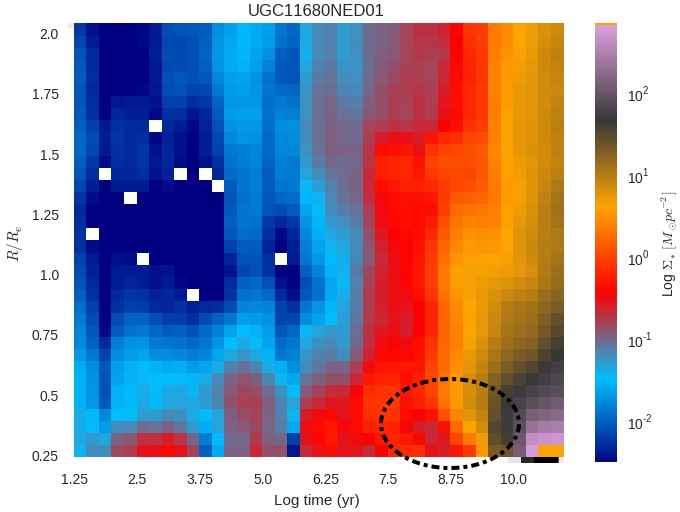
\includegraphics[scale=0.5]{figure_1.png}
  \caption[Densidad de masa estelar superficial, que define el mapa de Historia de Formación Estelar de UGC11680]{Densidad de masa estelar superficial, que define el mapa de Historia de Formación Estelar  de UGC11680. Se colocó un círculo punteado alrededor de la zona que tiene un ``corte'' en el gradiente de color, lo que implica un apagado que corre diagonalmente desde el centro galáctico hasta recorrer las zonas externas de la misma. Este corte no se observa en los promedios que se analizarán en la siguiente sección}
  \label{sfh_ugc11680}
\end{figure}


\noindent El resultado final, la historia de formación estelar espacialmente resuelta, dado por la densidad de masa estelar superficial o simplemente el mapa $SFH(t,R)$ para UGC11680, será el principal objeto de nuestro análisis. En la figura \ref{sfh_ugc11680}
el eje de las $X$ es la edad de las SSP a escala logarítmica, comienza con $\sim$ 14 Gyrs (la edad mas temprana de las SSPs utilizadas)
en el principio de la época cosmológica hasta el presente o tiempo actual que aquí definimos como tiempo cero.



\bigskip

\noindent Aunque no los utilizaremos, es interesante lo que muestran  las Figuras \ref{mass_SFH} y \ref{lum_SFH}. Estas muestran los mapas de la distribución espacial en luz (banda V) y densidad superficial de masa de la galaxia UG11680  para cada edad comprendida dentro de la plantilla SSSp utilizada. Si dividiéramos por el intervalo temporal tendríamos la tasa de formación estelar a cada tiempo. Se aprecia que a edades tempranas había mas formación estelar en el centro y más en las partes externas en edades recientes.



\begin{figure}
  \centering
    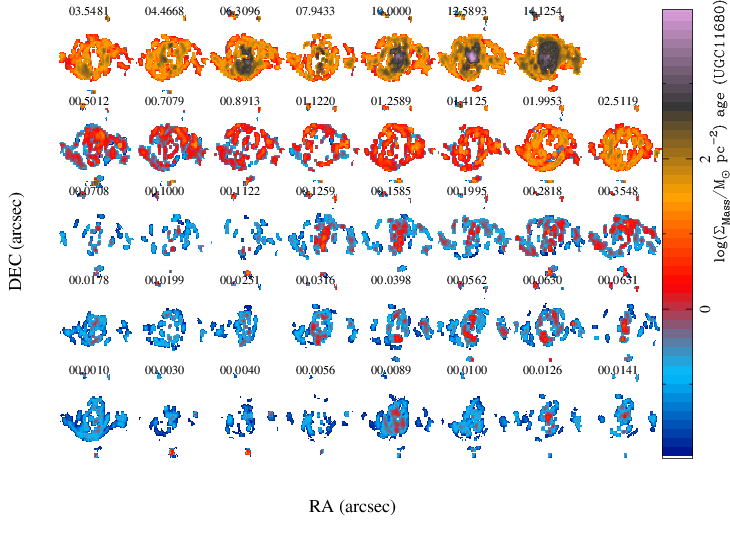
\includegraphics[scale=0.5]{Converted_file_73ee484d.png}
  \caption[Mapas de Densidad de masa superficial]{Mapas de densidad de masa estelar temporal cumulativa para UGC11680 antes de la compresión de los ejes $XY$ . La lectura de ellos comienza en la esquina superior derecha y termina en la esquina inferior izquierda}
  \label{mass_SFH}
\end{figure}

\noindent
\begin{figure}
  \centering
    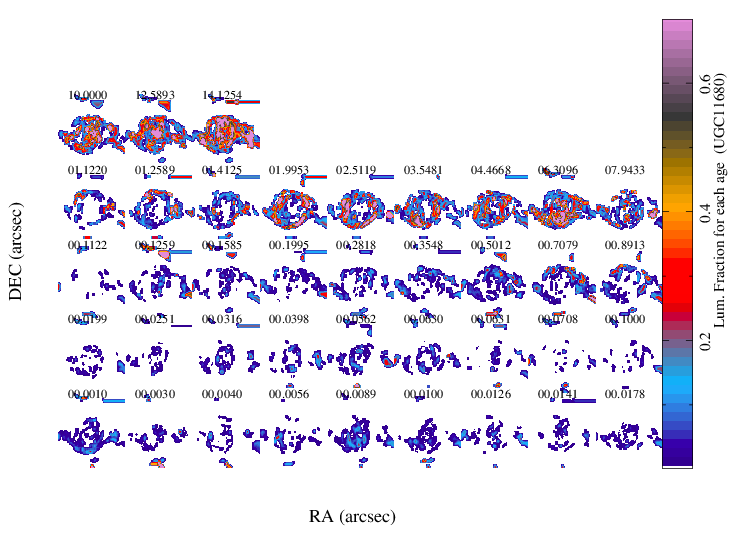
\includegraphics[scale=0.4]{18UGC11680_proc_elinesUGC11680_pruebas.png}
  \caption[Mapas de densidad superficial de luminosidad para UGC11680]{Disposición de mapas de luminosidad superficial para UGC11680 para cada SSP. Estos mapas temporales inician desde la esquina superior derecha y terminan en la esquina inferior izquierda.}
  \label{lum_SFH}
\end{figure}


\bigskip

\noindent Es importante aclarar que no existe acuerdo en la semántica de la palabra ``Historia'' en estudios de síntesis espectral. El mismo término puede ser utilizado de muchas formas en la literatura, siempre refiriéndose a alguna  medida de como la formación estelar evoluciona en el tiempo, pero cuantitativamente variando desde estimados en la edad promedio a mediciones de formación ``reciente'' (donde reciente puede ser cualquier cosa entre $\sim$ 10 Myrs a unos Gyrs, dependiendo de los trazadores). Además de las diferentes escalas de tiempo, diferentes índices pueden ser usados para medir la historia de formación estelar, tal como la luminosidad \citep{cid2013_1} o masa asociada a las estrellas dado un intervalo de edad, en forma cumulativa o diferencial, etc. Sin embargo, en este trabajo, siempre nos referiremos a la historia de formación estelar usando la densidad de masa estelar.

\bigskip


\noindent La riqueza de información de este mapa es de suma importancia y muestra claras diferencias entre galaxias o promedios de ellas; además, el mapa $SFH$ de la Figura \ref{sfh_ugc11680} nos da una representación bidimensional
de la producción de masa estelar en densidad de masa a tiempo dado. Las zonas menos densas representan desde una muy baja hasta nula formación estelar, mientras que las zonas más densas, sobre todo cerca del centro, nos da un un ensamblaje alto.

\bigskip

\noindent Observamos entonces que el mapa ya nos da indicios de ensamblaje ``dentro fuera'' para UGC11680. Marcamos con un círculo punteado la zona cerca de la parte central en donde se cambia de densidad, en forma de ``corte'' diagonal a edades tempranas $\sim$ 4 Gyrs (o altos \textsl{redshifts}) . Observamos también que la galaxia ensambló prácticamente toda su masa en aproximadamente $\sim$ 9 Gyrs.
Nótese también que la galaxia tiene moderados brotes de formación estelar en su centro y cerca de sus zonas medias,
y las partes externas prácticamente ya no forma estrellas a épocas actuales. Sin embargo, esto es un resultado cualitativo y corresponde al siguiente capitulo analizar la historia de formación estelar cuantitativamente.

\bigskip



\noindent En este capítulo se mostró que el polvo no enrojece lo suficiente a esta galaxia y que su tasa de formación estelar
esta por debajo de la secuencia principal de galaxias que forman estrellas.
Se analizó el proceso para obtener el mapa $SFH(t,R)$, es decir, la historia de formación estelar espacialmente resuelta de UGC11680.
En lo restante, analizaremos este mapa, comparándolo con diferentes mapas promediados, para que cualitativamente,
decidamos en cual de estos encaja mejor y así dar algunas hipótesis del apagado estelar.









 % The \citep command functions as follows:
 %   \citept{key} ==>>                Jones et al. (1990)
 %   \citept*{key} ==>>               Jones, Baker, and Smith (1990)
 %   \citepp{key} ==>>                (Jones et al., 1990)
 %   \citepp*{key} ==>>               (Jones, Baker, and Smith, 1990)
 %   \citepp[chap. 2]{key} ==>>       (Jones et al., 1990, chap. 2)
 %   \citepp[e.g.][]{key} ==>>        (e.g. Jones et al., 1990)
 %   \citepp[e.g.][p. 32]{key} ==>>   (e.g. Jones et al., p. 32)
 %   \citepauthor{key} ==>>           Jones et al.
 %   \citepauthor*{key} ==>>          Jones, Baker, and Smith
 %   \citepyear{key} ==>>             1990





%%%%%%%%%%%%%%%%%%%%%%%%%%%%%%%%%%%%%%%%%%%%%%%%%%%%%%%%%%%%%%%%%%%%%%%%%
%                          Descripción de la planta                     %
%%%%%%%%%%%%%%%%%%%%%%%%%%%%%%%%%%%%%%%%%%%%%%%%%%%%%%%%%%%%%%%%%%%%%%%%%






%%%%%%%%%%%%%%%%%%%%%%%%%%%%%%%%%%%%%%%%%%%%%%%%%%%%%%%%%%%%%%%%%%%%%%%%%
%                          Modelado                                     %
%%%%%%%%%%%%%%%%%%%%%%%%%%%%%%%%%%%%%%%%%%%%%%%%%%%%%%%%%%%%%%%%%%%%%%%%%

%%%%%%%%Tabla Nombres de parámetros



%%%%%%%%%%%%%%%%%%%%%%%%%%%%%%%%%%%%%%%%%%%%%%%%%%%%%%%%%%%%%%%%%%%%%%%%%
%                          Subsección
%%%%%%%%%%%%%%%%%%%%%%%%%%%%%%%%%%%%%%%%%%%%%%%%%%%%%%%%%%%%%%%%%%%%%%%%%
